%Use one of the two documentclass lines depending on the aspect ratio needed
% for 4x3 aspect ratio slides
%\documentclass{beamer}
%for 16x9 (modern wide screen) aspect ratio slides
\documentclass[aspectratio=169,8pt]{beamer}

% Oxford Maths theming
\setbeamertemplate{footline}[page number]
\usetheme{mytemplate}
\graphicspath{ {./figures/} {../../output/figures/} }
\definecolor{unil-blue}{RGB}{43,100,246}
\definecolor{success-green}{RGB}{46,125,50}
\definecolor{warning-orange}{RGB}{230,126,34}
\usepackage{amssymb,amsmath}
\usepackage{subfig}
\usepackage{minted}
\usepackage{hyperref}
\usepackage[utf8]{inputenc}
\usepackage[T1]{fontenc}
\usepackage{amsmath}
\usepackage{amssymb}
\usepackage{graphicx}
\usepackage{booktabs}
\usepackage{tikz}
\usepackage{xcolor}

% Set Info
\title[Data Science and Advanced Programming] %short version of title for slide footer
{\large IDENTIFYING KEY SOCIOECONOMIC DETERMINANTS OF INCOME INEQUALITY\\ A Machine Learning Approach Using World Bank Data} %full title for titlepage
\author{Benoit R. Goye}
\date[December 2025]  %short date for slide footer
{Data Science and Advanced Programming \(|\) December 2025} %main date for title page %can overload it to show, say 'Conference X, Date Y'

%Slides
\begin{document}

    % Title
    \begin{frame}[plain]
        \titlepage{}
    \end{frame}

    \begin{frame}{The Challenge of Income Inequality}
        \framesubtitle{Introduction \& Motivation}
        \begin{columns}[T]
            \column{0.5\textwidth}
            \begin{block}{Why it matters}
                \begin{itemize}
                    \scriptsize
                    \item Rising inequality $\rightarrow$ reduced social mobility
                    \item Political polarization
                    \item Slower economic growth
                    \item GINI coefficient: 0-100
                \end{itemize}
            \end{block}

            \column{0.5\textwidth}
            \begin{block}{Key questions}
                \begin{itemize}
                    \scriptsize
                    \item Which policy levers reduce inequality?
                    \item Are drivers universal or context-dependent?
                    \item Can we predict inequality accurately?
                \end{itemize}
            \end{block}
        \end{columns}

        \vspace{0.3cm}
        \begin{alertblock}{Traditional challenges}
            \scriptsize
            Non-linear relationships | High-dimensional data | Missing values (developing countries)
        \end{alertblock}
    \end{frame}

    \begin{frame}{Research Questions}
        \framesubtitle{Introduction \& Motivation}
        \begin{block}{RQ1: Feature Importance}
            Which socioeconomic indicators are the \textbf{strongest predictors} of GINI coefficients?
        \end{block}

        \begin{block}{RQ2: Cross-Model Consistency}
            Are predictor rankings \textbf{consistent across different ML algorithms}?
        \end{block}

        \begin{block}{RQ3: Predictive Performance}
            How well can we \textbf{predict inequality} across different contexts?
        \end{block}

        \vspace{0.3cm}
        \begin{alertblock}{Contribution}
            Data-driven approach using 5 ML algorithms to explore inequality drivers while implementing advanced optimization techniques
        \end{alertblock}
    \end{frame}

    \begin{frame}{Data: World Bank Database (2000-2023)}
        \framesubtitle{Data \& Methodology}
        \begin{columns}[T]
            \column{0.5\textwidth}
            \begin{block}{Target Variable}
                GINI coefficient | $\sim$1,800 country-year observations
            \end{block}

            \vspace{0.2cm}
            \begin{block}{$\sim$60 Predictor Variables}
                \scriptsize
                \begin{enumerate}
                    \item Economic (GDP, trade, inflation)
                    \item Demographics (population, urbanization)
                    \item Human development (health, education)
                    \item Labor market (employment rates)
                    \item Infrastructure (electricity, internet)
                    \item Governance (gender parity)
                \end{enumerate}
            \end{block}

            \column{0.5\textwidth}
            \begin{block}{Preprocessing}
                \begin{itemize}
                    \scriptsize
                    \item KNN imputation (k=5)
                    \item Exclude features $>$50\% missing
                    \item 80-20 train-test split
                    \item 5-fold cross-validation
                \end{itemize}
            \end{block}

            \vspace{0.2cm}
            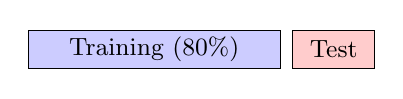
\begin{tikzpicture}[scale=0.8]
                \draw[fill=blue!20] (0,0) rectangle (4,0.6);
                \node at (2,0.3) {\small Training (80\%)};
                \draw[fill=red!20] (4.2,0) rectangle (5.5,0.6);
                \node at (4.85,0.3) {\small Test};
            \end{tikzpicture}
        \end{columns}
    \end{frame}

    \begin{frame}{Five Tree-Based Algorithms}
        \framesubtitle{Data \& Methodology}
        \begin{table}
            \centering
            \small
            \begin{tabular}{llp{5cm}}
                \toprule
                \textbf{Model} & \textbf{Type} & \textbf{Key Feature} \\
                \midrule
                Decision Tree & Baseline & Single tree, recursive partitioning \\
                \midrule
                Random Forest & Ensemble & Bootstrap + random features \\
                & (Bagging) & Reduces variance \\
                \midrule
                Gradient Boosting & Ensemble & Sequential fitting of residuals \\
                & (Boosting) & Reduces bias \\
                \midrule
                XGBoost & Advanced & Regularized objective \\
                & Boosting & 2nd-order optimization \\
                \midrule
                LightGBM & Advanced & Histogram-based + GOSS \\
                & Boosting & Computational efficiency \\
                \bottomrule
            \end{tabular}
        \end{table}

        \vspace{0.2cm}
        \textbf{Hyperparameters:} 200 estimators, learning rate 0.05, max depth 5-10, regularization
    \end{frame}

    \begin{frame}{Statistical Validation Framework}
        \framesubtitle{Data \& Methodology}

        \begin{block}{1. Bootstrap Confidence Intervals}
            \scriptsize
            Train each model 100 times on bootstrap samples. Compute 95\% CI. Parallel processing (6$\times$ speedup).
        \end{block}

        \vspace{0.1cm}
        \begin{block}{2. Permutation Importance Tests}
            \scriptsize
            Randomly permute features (50 permutations). Measure drop in $R^2$. One-sample t-test ($\alpha = 0.05$).
        \end{block}

        \vspace{0.1cm}
        \begin{block}{3. Cross-Model Consistency}
            \scriptsize
            Spearman rank correlations between models. High $\rho > 0.7$ $\rightarrow$ robust rankings.
        \end{block}

        \vspace{0.2cm}
        \begin{alertblock}{Goal}
            Ensure feature importance rankings are statistically robust and consistent
        \end{alertblock}
    \end{frame}

    \begin{frame}{Segmentation Analysis}
        \framesubtitle{Data \& Methodology}
        \begin{columns}[T]
            \column{0.55\textwidth}
            \textbf{Testing context-dependence:}

            \vspace{0.2cm}
            \textbf{By Income Level:}
            \begin{itemize}
                \item Low income
                \item Lower-middle income
                \item Upper-middle income
                \item High income
            \end{itemize}

            \vspace{0.2cm}
            \textbf{By Geographic Region:}
            \begin{itemize}
                \scriptsize
                \item East Asia \& Pacific
                \item Europe \& Central Asia
                \item Latin America \& Caribbean
                \item Middle East \& North Africa
                \item South Asia
                \item Sub-Saharan Africa
            \end{itemize}

            \column{0.45\textwidth}
            \begin{center}
                \includegraphics[width=\textwidth]{segment_performance.png}
            \end{center}

            \vspace{0.2cm}
            \begin{alertblock}{Key Question}
                Are inequality drivers universal or context-specific?
            \end{alertblock}
        \end{columns}
    \end{frame}

    \begin{frame}{Model Performance: Ensemble Methods Excel}
        \framesubtitle{Results}
        \begin{columns}[T]
            \column{0.5\textwidth}
            \begin{table}
                \centering
                \small
                \begin{tabular}{lcc}
                    \toprule
                    \textbf{Model} & \textbf{Test $R^2$} & \textbf{RMSE} \\
                    \midrule
                    Decision Tree & \textcolor{red}{0.787} & 3.89 \\
                    Random Forest & 0.890 & 2.79 \\
                    Gradient Boosting & \textcolor{success-green}{\textbf{0.905}} & 2.58 \\
                    XGBoost & \textcolor{success-green}{\textbf{0.902}} & 2.62 \\
                    LightGBM & 0.895 & 2.72 \\
                    \bottomrule
                \end{tabular}
            \end{table}

            \vspace{0.2cm}
            \begin{block}{Key Findings}
                \scriptsize
                Ensembles outperform single tree. GB \& XGBoost: $R^2 > 0.90$. Good generalization.
            \end{block}

            \column{0.5\textwidth}
            \begin{center}
                \includegraphics[width=\textwidth,height=0.65\textheight,keepaspectratio]{comprehensive_comparison.png}
            \end{center}
        \end{columns}
    \end{frame}

    \begin{frame}{Top 10 Features: Infrastructure Dominates}
        \framesubtitle{Results}
        \begin{columns}[T]
            \column{0.35\textwidth}
            \begin{table}
                \centering
                \scriptsize
                \begin{tabular}{rlr}
                    \toprule
                    \textbf{Rank} & \textbf{Feature} & \textbf{Imp.} \\
                    \midrule
                    1 & Rural electricity & \textcolor{success-green}{\textbf{0.288}} \\
                    2 & Total electricity & 0.067 \\
                    3 & Trade openness & 0.034 \\
                    4 & Renewable energy & 0.031 \\
                    5 & Forest area & 0.027 \\
                    6 & Agriculture \% GDP & 0.026 \\
                    7 & Exports \% GDP & 0.024 \\
                    8 & Gender labor gap & 0.023 \\
                    9 & Rural population & 0.023 \\
                    10 & Services employ. & 0.022 \\
                    \bottomrule
                \end{tabular}
            \end{table}

            \column{0.65\textwidth}
            \begin{center}
                \includegraphics[width=\textwidth,height=0.6\textheight,keepaspectratio]{feature_importance.png}
            \end{center}
        \end{columns}

        \begin{alertblock}{Implication}
            Inequality driven by \textbf{small subset} of critical factors
        \end{alertblock}
    \end{frame}

    \begin{frame}{Statistical Significance Confirmed}
        \framesubtitle{Results}
        \begin{columns}[T]
            \column{0.5\textwidth}
            \begin{center}
                \includegraphics[width=\textwidth,height=0.5\textheight,keepaspectratio]{statistical_tests_bootstrap.png}
            \end{center}

            \begin{block}{Bootstrap CI}
                \scriptsize
                All top 10: 95\% CI excludes zero. High stability.
            \end{block}

            \column{0.5\textwidth}
            \begin{center}
                \includegraphics[width=\textwidth,height=0.5\textheight,keepaspectratio]{statistical_tests_consistency.png}
            \end{center}

            \begin{block}{Cross-Model}
                \scriptsize
                GB vs XGBoost: $\rho = 0.84$. Core drivers consistent.
            \end{block}
        \end{columns}

        \vspace{0.15cm}
        \begin{alertblock}{Conclusion}
            Top predictors are \textbf{robust} across resampling, algorithms, and tests
        \end{alertblock}
    \end{frame}

    \begin{frame}{Context Matters: Income-Level Heterogeneity}
        \framesubtitle{Results}
        \begin{columns}[T]
            \column{0.5\textwidth}
            \begin{center}
                \includegraphics[width=\textwidth,height=0.5\textheight,keepaspectratio]{segmentation_income_performance.png}
            \end{center}

            \begin{block}{Performance}
                \scriptsize
                High: $R^2 = 0.86$-$0.88$ | Upper-mid: $0.85$-$0.91$ | Lower-mid: $0.81$-$0.86$ | Low: $0.69$-$0.73$
            \end{block}

            \column{0.5\textwidth}
            \begin{center}
                \includegraphics[width=\textwidth,height=0.5\textheight,keepaspectratio]{segmentation_income_features.png}
            \end{center}

            \begin{block}{Top Drivers}
                \scriptsize
                \textbf{Low:} Infrastructure | \textbf{Mid:} Urbanization | \textbf{High:} Trade \& labor
            \end{block}
        \end{columns}

        \vspace{0.15cm}
        \begin{alertblock}{Policy Implication}
            \textbf{Tailored interventions} needed by development stage
        \end{alertblock}
    \end{frame}

    \begin{frame}{Regional Heterogeneity: Geography Matters}
        \framesubtitle{Results}
        \begin{columns}[T]
            \column{0.5\textwidth}
            \begin{center}
                \includegraphics[width=\textwidth,height=0.5\textheight,keepaspectratio]{segmentation_regional_performance.png}
            \end{center}

            \begin{block}{Performance by Region}
                \scriptsize
                Europe \& Central Asia: Highest $R^2$ | Latin America: Moderate | Sub-Saharan Africa: Lower
            \end{block}

            \column{0.5\textwidth}
            \begin{center}
                \includegraphics[width=\textwidth,height=0.5\textheight,keepaspectratio]{segmentation_regional_features.png}
            \end{center}

            \begin{block}{Different Drivers}
                \scriptsize
                Region-specific factors. Historical \& institutional differences matter.
            \end{block}
        \end{columns}

        \vspace{0.15cm}
        \begin{alertblock}{Key Insight}
            Inequality determinants vary by \textbf{income level} and \textbf{geography}
        \end{alertblock}
    \end{frame}

    \begin{frame}{Model Diagnostics: Strong Performance}
        \framesubtitle{Results}
        \begin{columns}[T]
            \column{0.5\textwidth}
            \begin{center}
                \includegraphics[width=\textwidth,height=0.5\textheight,keepaspectratio]{predictions_plot.png}
            \end{center}

            \begin{block}{Predicted vs Actual}
                \scriptsize
                Strong $R > 0.90$. GINI 20-45: excellent. GINI $>$ 50: underprediction.
            \end{block}

            \column{0.5\textwidth}
            \begin{center}
                \includegraphics[width=\textwidth,height=0.5\textheight,keepaspectratio]{error_analysis.png}
            \end{center}

            \begin{block}{Error Analysis}
                \scriptsize
                Errors near zero. Few outliers. Consistent across models.
            \end{block}
        \end{columns}

        \vspace{0.15cm}
        \begin{alertblock}{Conclusion}
            Models generalize well but struggle with extreme outliers
        \end{alertblock}
    \end{frame}

    \begin{frame}{Computational Performance: 3-5$\times$ Speedup}
        \framesubtitle{Implementation \& Optimization}
        \textbf{Parallel Processing Strategies:}

        \begin{table}
            \centering
            \small
            \begin{tabular}{llcc}
                \toprule
                \textbf{Component} & \textbf{Method} & \textbf{Before} & \textbf{After} \\
                \midrule
                Data collection & ThreadPoolExecutor (6 workers) & 12 min & \textcolor{success-green}{\textbf{2 min}} \\
                Bootstrap tests & joblib Parallel (n\_jobs=-1) & 60 sec & \textcolor{success-green}{\textbf{10 sec}} \\
                Model training & scikit-learn parallelization & 25 sec & \textcolor{success-green}{\textbf{5 sec}} \\
                \midrule
                \textbf{Total pipeline} & Combined optimizations & \textbf{25-35 min} & \textcolor{success-green}{\textbf{5-7 min}} \\
                \bottomrule
            \end{tabular}
        \end{table}

        \vspace{0.3cm}
        \begin{columns}[T]
            \column{0.5\textwidth}
            \textbf{Intelligent Caching:}
            \begin{itemize}
                \item SHA256 hash validation
                \item Auto cache invalidation
                \item 60-100$\times$ speedup on reruns
            \end{itemize}

            \column{0.5\textwidth}
            \textbf{Impact:}
            \begin{itemize}
                \item \textcolor{success-green}{\textbf{6$\times$ faster}} data collection
                \item \textcolor{success-green}{\textbf{6$\times$ faster}} bootstrap
                \item \textcolor{success-green}{\textbf{5$\times$ faster}} training
            \end{itemize}
        \end{columns}
    \end{frame}

    \begin{frame}{Software Engineering Best Practices}
        \framesubtitle{Implementation \& Optimization}
        \begin{columns}[T]
            \column{0.5\textwidth}
            \begin{block}{Modular Architecture}
                \scriptsize
                9-stage pipeline: Data collection $\rightarrow$ Preprocessing $\rightarrow$ Training $\rightarrow$ Prediction $\rightarrow$ Evaluation $\rightarrow$ Comparison $\rightarrow$ Segmentation $\rightarrow$ Statistical tests $\rightarrow$ Report generation
            \end{block}

            \vspace{0.2cm}
            \begin{block}{Execution Modes}
                \begin{itemize}
                    \scriptsize
                    \item \textbf{Quick:} Full pipeline (default)
                    \item \textbf{Fast:} 2015-2023 only
                    \item \textbf{Optimized:} Hyperparameter tuning
                    \item \textbf{Custom:} Fine-grained control
                \end{itemize}
            \end{block}

            \column{0.5\textwidth}
            \begin{block}{Quality Assurance}
                \begin{itemize}
                    \scriptsize
                    \item Type annotations
                    \item Comprehensive docstrings
                    \item Data hash validation
                    \item Deterministic results (seed=42)
                    \item Dependency management
                \end{itemize}
            \end{block}

            \vspace{0.2cm}
            \begin{block}{Reproducibility}
                \begin{itemize}
                    \scriptsize
                    \item Git version control
                    \item Automated caching
                    \item Complete documentation
                    \item Public code repository
                \end{itemize}
            \end{block}
        \end{columns}
    \end{frame}

    \begin{frame}{Key Findings Summary}
        \framesubtitle{Conclusions \& Policy Implications}

        \begin{block}{1. Predictive Power: Ensemble methods achieve $R^2 > 0.90$}
            \begin{itemize}
                \scriptsize
                \item Inequality is highly predictable from socioeconomic factors
                \item Gradient Boosting \& XGBoost perform best
            \end{itemize}
        \end{block}

        \begin{block}{2. Infrastructure Dominates: Rural electricity access (imp. 0.304)}
            \begin{itemize}
                \scriptsize
                \item 5$\times$ more important than any other feature
                \item Composite measure of development, institutions, connectivity
            \end{itemize}
        \end{block}

        \begin{block}{3. Robust Core Drivers: Trade, economic structure, gender gaps}
            \begin{itemize}
                \scriptsize
                \item Consistent across all five models
                \item Statistically significant (bootstrap \& permutation tests)
            \end{itemize}
        \end{block}

        \begin{block}{4. Context-Dependent: Different drivers at different income levels}
            \begin{itemize}
                \scriptsize
                \item Low income: Basic infrastructure | Middle: Urbanization | High: Trade \& labor markets
            \end{itemize}
        \end{block}
    \end{frame}

    \begin{frame}{Policy Implications}
        \framesubtitle{Conclusions \& Policy Implications}
        \textbf{Three priority areas for reducing inequality:}

        \begin{block}{1. Expand Infrastructure Access}
            \begin{itemize}
                \item Particularly rural electricity connectivity
                \item Enables economic opportunities \& education access
                \item Signals institutional capacity for service delivery
            \end{itemize}
        \end{block}

        \begin{block}{2. Promote Inclusive Labor Markets}
            \begin{itemize}
                \item Reduce gender labor gaps
                \item Increase labor force participation (especially women)
                \item Address youth unemployment
            \end{itemize}
        \end{block}

        \begin{block}{3. Manage Structural Transformation}
            \begin{itemize}
                \item Progressive taxation \& social insurance
                \item Education access that scales with industrial demands
                \item Minimum wage floors to prevent wage compression
            \end{itemize}
        \end{block}
    \end{frame}

    \begin{frame}{Limitations \& Future Directions}
        \begin{columns}[T]
            \column{0.5\textwidth}
            \textbf{Limitations:}
            \begin{itemize}
                \item \textbf{Prediction not causation}
                \begin{itemize}
                    \scriptsize
                    \item Need IV, DiD, RDD for causal effects
                \end{itemize}
                \item Missing data imputation uncertainty
                \item Stationarity assumption
                \begin{itemize}
                    \scriptsize
                    \item Relationships may change over time
                \end{itemize}
                \item Omitted variables
                \begin{itemize}
                    \scriptsize
                    \item Institutional quality, tax progressivity
                \end{itemize}
            \end{itemize}

            \column{0.5\textwidth}
            \textbf{Future Research:}
            \begin{enumerate}
                \item \textbf{Causal inference}
                \begin{itemize}
                    \scriptsize
                    \item Double ML, causal forests
                \end{itemize}
                \item \textbf{Additional data}
                \begin{itemize}
                    \scriptsize
                    \item Satellite imagery
                    \item Institutional quality measures
                    \item Alternative inequality metrics
                \end{itemize}
                \item \textbf{Methodological advances}
                \begin{itemize}
                    \scriptsize
                    \item SHAP values for interactions
                    \item Panel methods with time-varying coefficients
                \end{itemize}
            \end{enumerate}
        \end{columns}

        \vspace{0.3cm}
        \begin{alertblock}{Bottom Line}
            ML complements traditional econometrics: prediction + pattern recognition vs. causal identification
        \end{alertblock}
    \end{frame}

    \begin{frame}{Contributions to Literature}
        \framesubtitle{Conclusions \& Policy Implications}
        \begin{columns}[T]
            \column{0.5\textwidth}
            \begin{block}{Methodological Contributions}
                \begin{itemize}
                    \scriptsize
                    \item First systematic comparison of 5 tree-based ML algorithms
                    \item Robust statistical validation framework
                    \item Advanced optimization (3-5$\times$ speedup)
                    \item Fully reproducible pipeline
                \end{itemize}
            \end{block}

            \vspace{0.2cm}
            \begin{alertblock}{Innovation}
                Combines ML prediction power with rigorous statistical validation
            \end{alertblock}

            \column{0.5\textwidth}
            \begin{block}{Substantive Contributions}
                \begin{itemize}
                    \scriptsize
                    \item Infrastructure as dominant predictor
                    \item Context-dependence quantified
                    \item High predictability ($R^2 > 0.90$)
                    \item Tailored policy recommendations
                \end{itemize}
            \end{block}

            \vspace{0.2cm}
            \begin{alertblock}{Impact}
                Data-driven evidence for targeted inequality reduction
            \end{alertblock}
        \end{columns}

        \vspace{0.2cm}
        \begin{center}
            \textbf{Data \& Code:} \textcolor{unil-blue}{Publicly available for replication}
        \end{center}
    \end{frame}

    \begin{frame}[plain]
        \usebeamertemplate{endpage}
    \end{frame}

    \begin{frame}
        \frametitle{APPENDIX}
        \framesubtitle{Txt \(|\) TxT}
        Txt
    \end{frame}

\end{document}
